In this chapter, we present a real-world validation of our coevolutionary approach using a swarm of physical e-puck robots. Unlike the simulation, the evolution in physical systems would become much harder as there would be numerous noises. Moreover, since the simulation could not model the exact dynamics (such as collision) in reality, in the physical coevolutionary experiments we still need to deal with uncertainties which will be discussed later in the implementation. Evolution on physical systems breaks the gap between simulation and reality and could bring us new insight on how to implement evolution in real world. Here we detail the implementation of a complete system for learning the aggregation behavior in Chapter~\ref{ch:swarm_simulation} with minimal human intervention, and discuss the results obtained. 

This chapter is organized as follows. Sec.~\ref{sec:experimental_setup} introduces the physical setup, including robot arena, robot platform and sensor implementation. Sec.~\ref{motion_capture_and_video_processing} details the motion capture and video processing. Sec.~\ref{pc_and_robot_programs} presents the programs executed by the robots and the machine. Sec.~\ref{sec:experimental_protocol} describes the experimental setup and protocol. Sec.~\ref{sec:experimental_results} discusses the results obtained. Sec.~\ref{sec:analysis_algorithm} analyzes the sensitivity of the coevolutionary approach for individual failures during the experiments. Sec.~\ref{sec:summary_swarm_physical} summaries the results obtained and discusses the findings.

\section{Physical Platform}\label{sec:experimental_setup_swarm_physical}
The physical platform, shown in Fig.~\ref{fig:physical_system_setup}, consists of an arena with robots (representing agents or replicas), a personal computer (PC) and an overhead camera. The PC runs the coevolutionary algorithm\footnote{The evolution of the model population could in principle be conducted on the on-board micro-controller of the e-puck, but running it on the PC reduces experimental time~\cite{Floreano1996}.}. It communicates with the replicas, issuing them with models to be executed, but does not exert any control over the other agents. The overhead camera supplies the PC with a video stream of the swarm. The PC performs video processing to obtain motion data about individual robots.
We will now detail these various components.

\begin{figure}[!t]
    \centering
    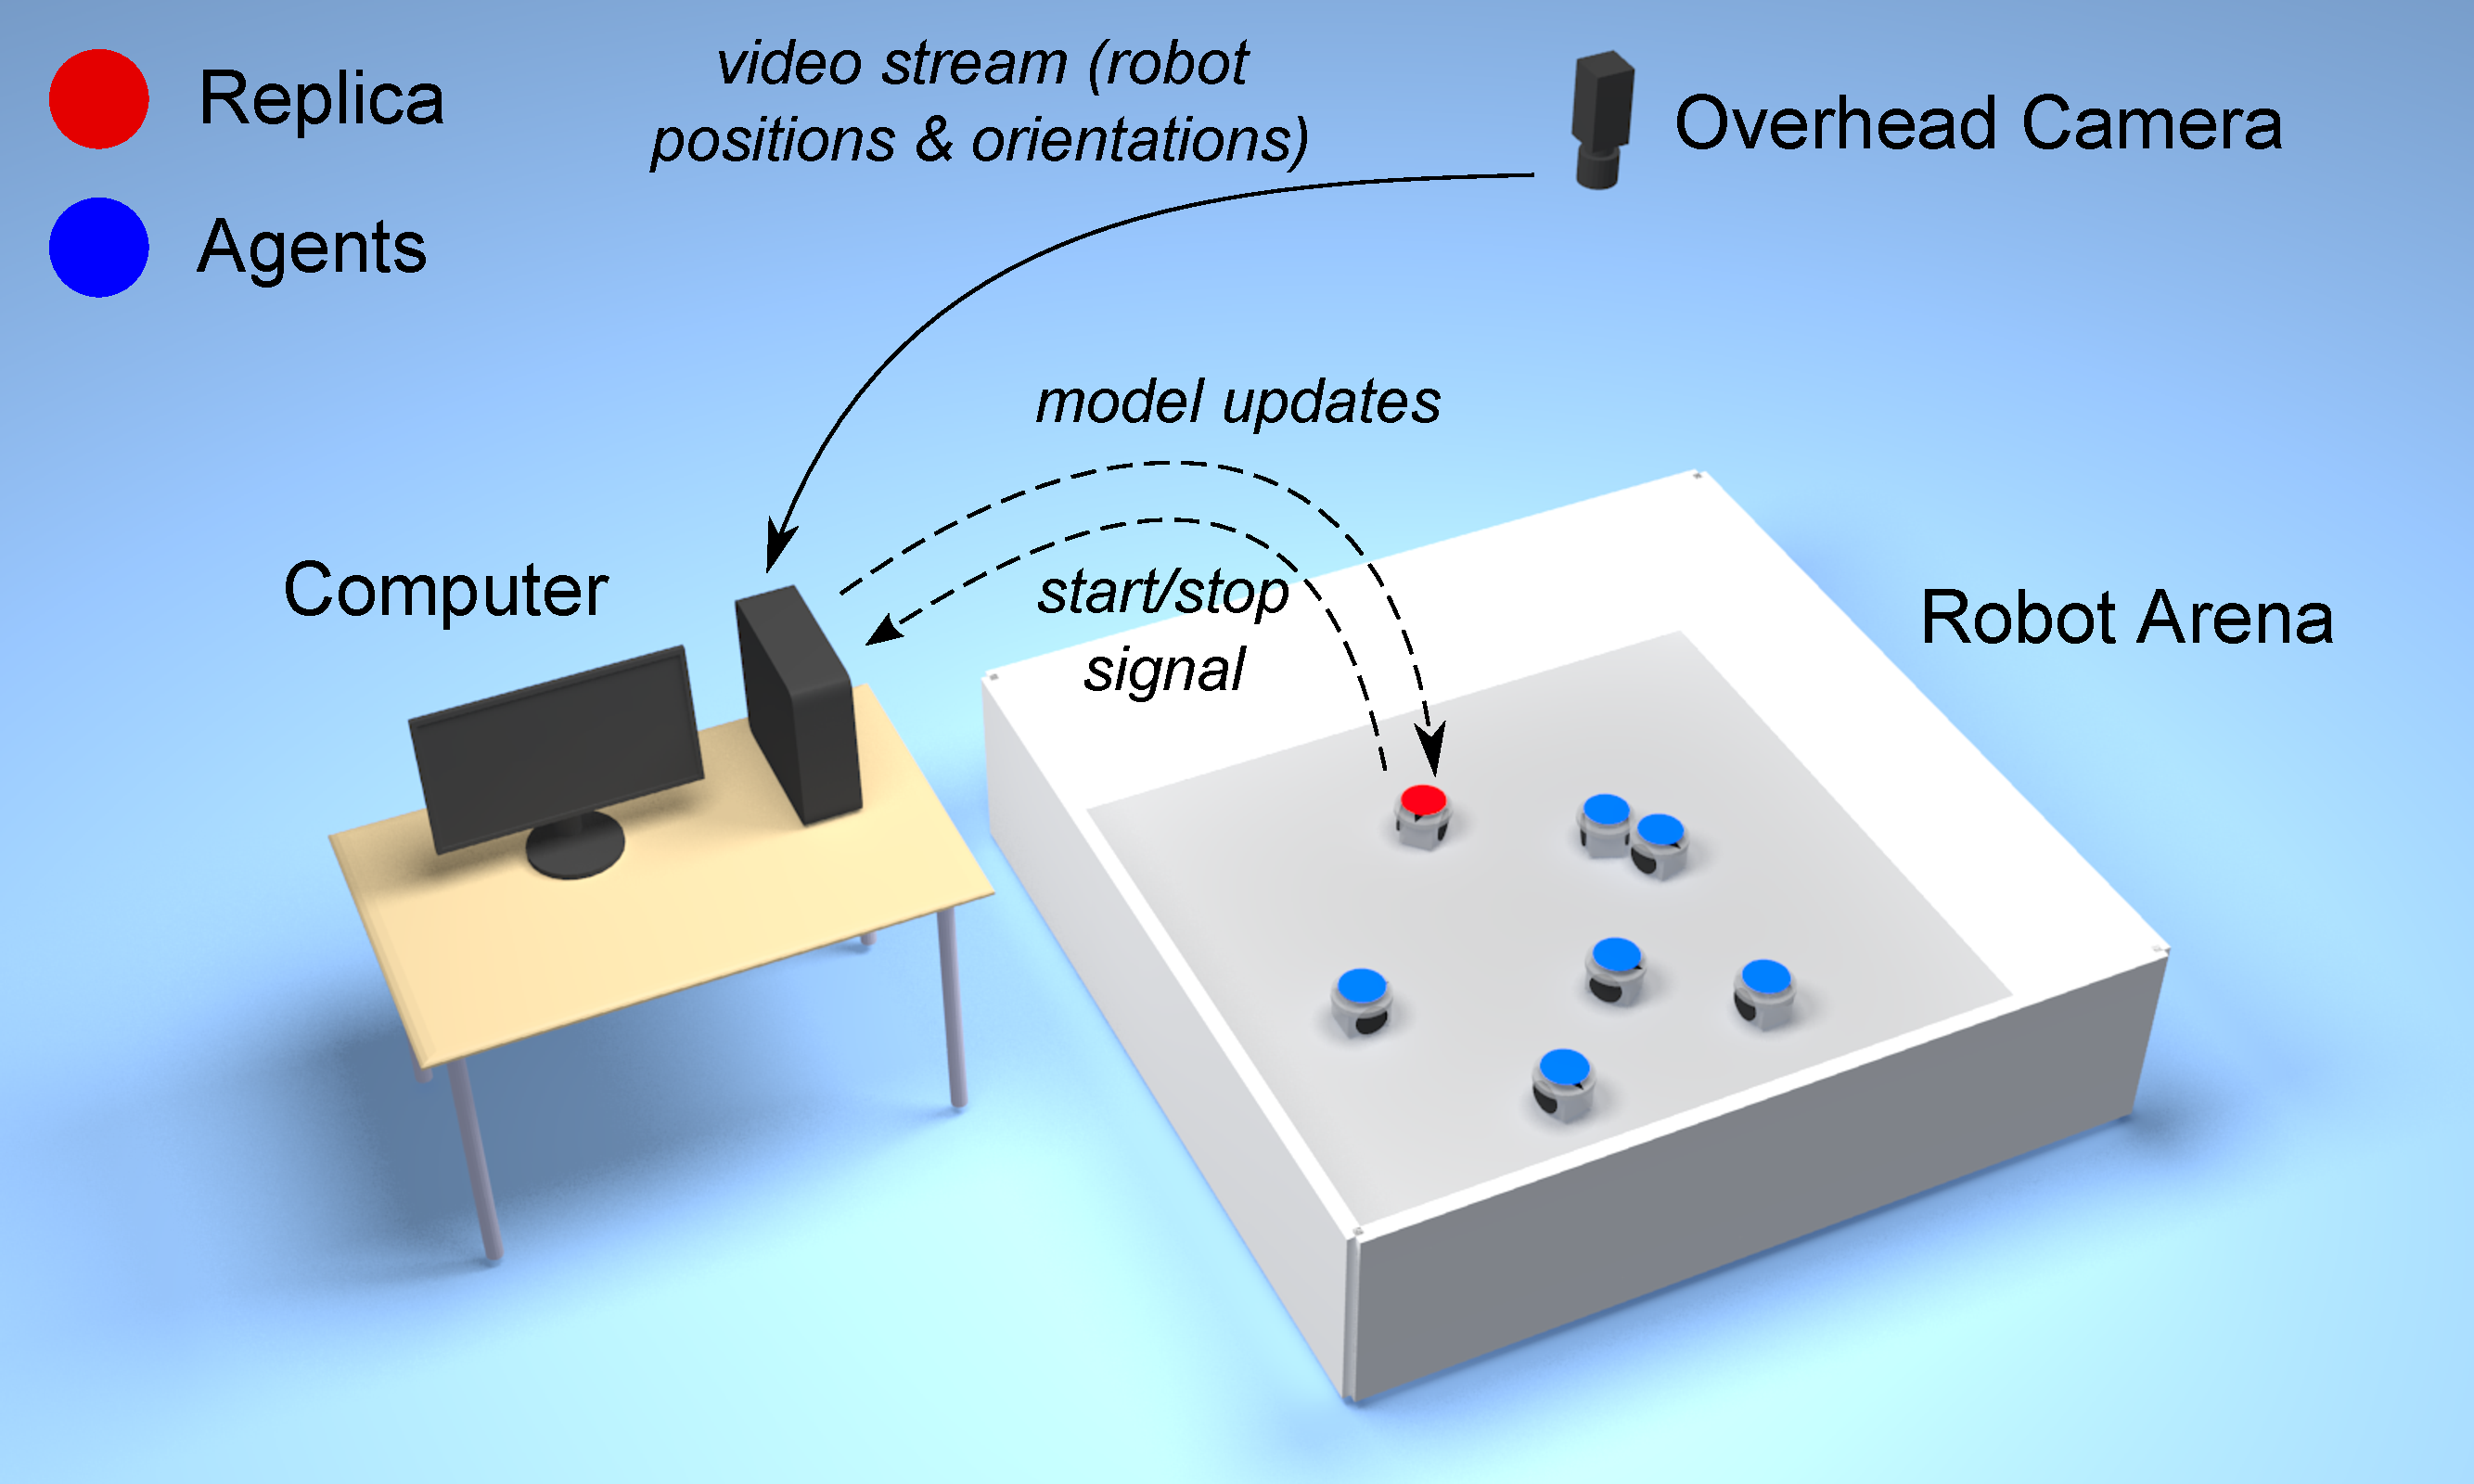
\includegraphics[width=3.5in]{physical_system_setup.pdf}
    \caption{The physical setup. }
    \label{fig:physical_system_setup}
\end{figure} 

\begin{figure}[!t]
	\centering
	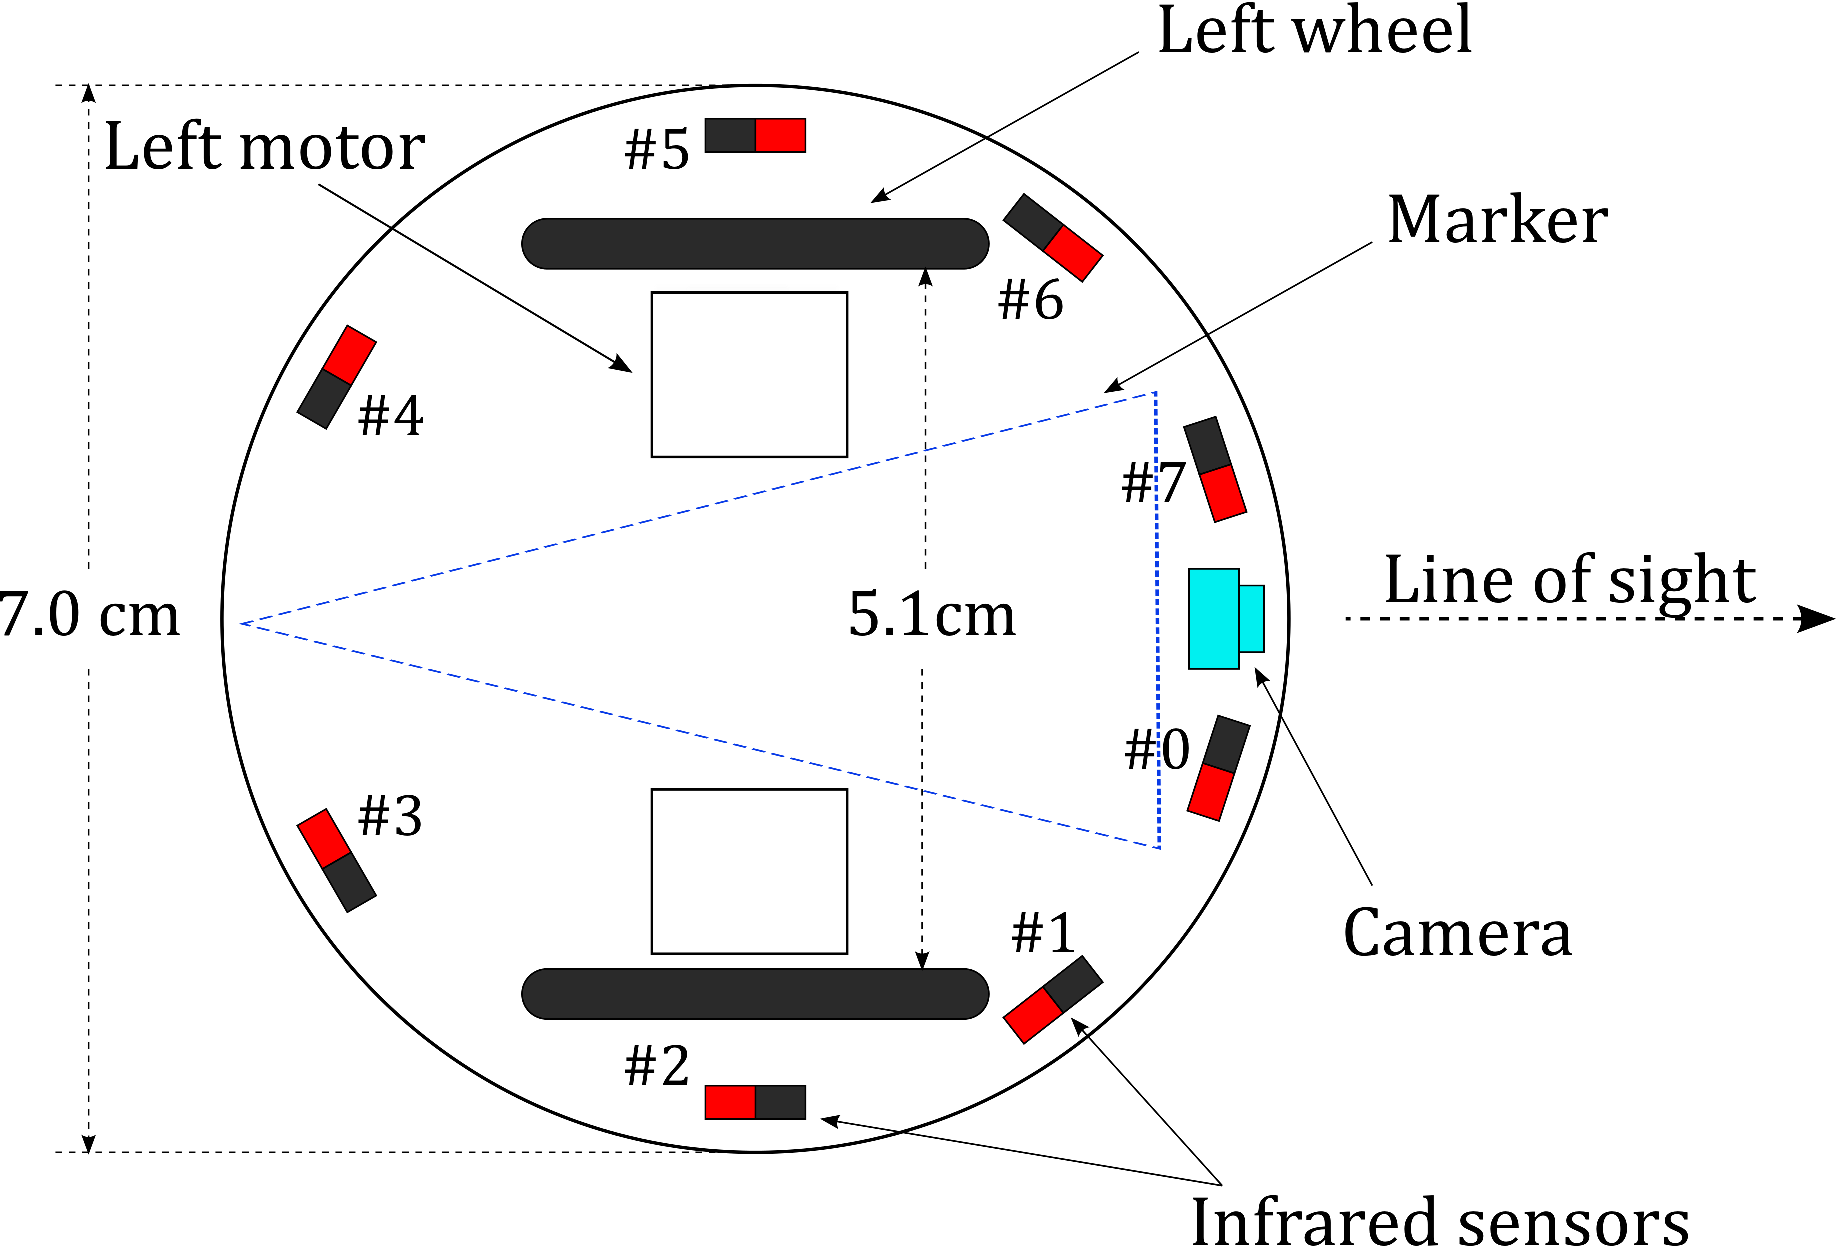
\includegraphics[width=3.5in]{drawing_epuck_schematic.pdf}
	\caption{Schematic top-view of an e-puck, indicating the locations of its motors, wheels, camera and infrared sensors. Note that the marker is pointing towards the robot's \emph{back}.}
	\label{fig:e_puck_schematic}
\end{figure}

\subsection{Robot Arena}

The robot arena was rectangular with sides $\unit[200]{cm} \times \unit[225]{cm}$, and bounded by walls $\unit[50]{cm}$ high. The floor had a light gray color, and the walls were painted white. 

\subsection{Robot Platform and Sensor Implementations}\label{sec:robot_platform_sensor_implementation}

\subsubsection{Robot Platform}
In Chapter~\ref{ch:swarm_simulation}, we presented the e-puck's shape and dimensions as a basis for the agents' embodiment in simulation. We now present further details about the e-puck relevant to our physical implementation. 

The e-puck has a directional camera located in its front. The resolution of the camera is up to $640\times480$, corresponding to the horizontal and vertical angle view of $56\degree$ and $48\degree$. The image is sub-sampled to $40\times15$ pixels due to the limited memory size of the on-board micro-controller, which is the Microchip dsPIC30F6014A with 8KB of RAM and 144 KB of flash memory. There are eight infrared proximity sensors around the body of the robot. These are only used for collision/wall avoidance in the physical coevolutions where the environment is bounded. In the e-puck, the light-of-sight sensor is implemented using the middle column of the pixels from the camera~\citep{Gauci2014_ijrr}. If any pixel of that column exceeds a certain threshold in its gray scale, the sensor outputs $1$; otherwise, it outputs $0$. A schematic top view of the e-puck, showing the sensors and actuators used, is shown in Fig.~\ref{fig:e_puck_schematic}.

\subsubsection{Sensor Implementations}

We implemented the line-of-sight sensor using the e-puck's directional camera, located at its front. For this purpose, we wrapped the robots in black `skirts' (see Fig.~\ref{fig:e-puck_body}) to make them distinguishable against the light-colored arena.  However, we use the camera in monochrome mode, and sub-sample the image to $40 \times 15$ pixels, due to the e-puck's limited memory (which cannot even store a single full-resolution image). While in principle the sensor could be implemented using one pixel, we used a column of pixels from a sub-sampled image to compensate for misalignment in the camera's vertical orientation. The gray values from these pixels were used to distinguish robots ($I=1$) against the arena ($I=0$). For more details about this sensor realization, see~\cite{Gauci2014_ijrr}.

We also used the e-puck's infrared sensors, for two reasons. Firstly, we observed that using only the line-of-sight sensor for aggregation often leads to robots becoming stuck against the walls of the arena, hindering the coevolutionary process. We therefore used the infrared sensors for wall avoidance, but in such a way as to not affect inter-robot interactions.
Secondly, before each trial, the robots dispersed themselves within the arena (behavior \textit{R1} in Sec.~\ref{pc_and_robot_programs}). In this case, we used the infrared sensors to avoid both robots and walls, making the dispersion process more efficient. In the following, we details the implementation of these two programs (\textit{disperse} program and~\textit{wall avoidance} program). 

1) The implementation of~\textit{disperse} program after a trial:

After finishing a trial, we disperse the robots for a while (which is equivalent to initial configuration for a new trial) in order to automate the coevolutionary learning process. This program consists of two behaviors---obstacle avoidance and disperse. The obstacle avoidance behavior is to prevent the robots colliding with other robots and the walls. In particular, before executing the disperse behavior, each robot detects whether some other objects (robots/walls) exist around it through emitting pulses of infrared light and measuring their reflections. If it detects something, it moves away from the objects through adjusting the linear and angular speed accordingly using a single-layer neural network controller. The obstacle avoidance behavior lasts for 3 seconds. In the disperse behavior, each robot is moving forward with a fixed linear speed while avoiding collisions with other robots and the walls. This behavior lasts for 5 seconds.

2) The implementation of~\textit{wall avoidance} program during a trial:

During a trial, in order to reduce the chances of robots getting stuck against the walls (note that the aggregation behavior was designed in an unbounded environment), we implemented the wall avoidance behavior, but in such a way as to not affect inter-robot interactions. In particular, when the robot detected the white walls using the infrared sensors or saw another robot ($I=1$) using the camera, it executed the same behavior. For example, for the agent, it would also turn on the spot when detecting the walls, which makes it easier to avoid the walls. However, the behavior of the replica depends on the model it is executing. Different from the Disperse program, the program of wall avoidance was only triggered when the value of any of the robot's infrared sensor was above a pre-set high threshold. This ensures that the value of the robot's infrared sensors when other robots (covered with a black 'skirt') were nearby was always below the threshold. Therefore, the wall avoidance program did not affect the aggregation of robots.

\section{Motion Capture and Video Processing}\label{motion_capture_and_video_processing_swarm_physical}

\subsection{Motion Capture}

To facilitate motion data extraction, we fitted robots with markers on their tops, consisting of a colored isosceles triangle on a circular white background. The triangle's color allowed for distinction between robots; we used blue triangles for all agents, and orange and purple triangles for the two replicas. The triangle's shape eased extraction of robots' orientations. Note that the orientation of the triangle is pointing to the backward of the e-puck robot so that it can be easily attached.

The robots' motion was captured using a GigE color camera (Basler Technologies), mounted around $\unit[300]{cm}$ above the ground. The camera's frame rate was set to $\unit[10]{fps}$. The video stream was fed to the PC, which performed video processing to extract motion data about individual robots (position and orientation). The size of the arena in the image is 
$\unit[700]{pixels} \times \unit[800]{pixels}$. An image of the arena is shown in Fig.~\ref{fig:robot_arena}.
%
\begin{figure}[!t]
    \centering
    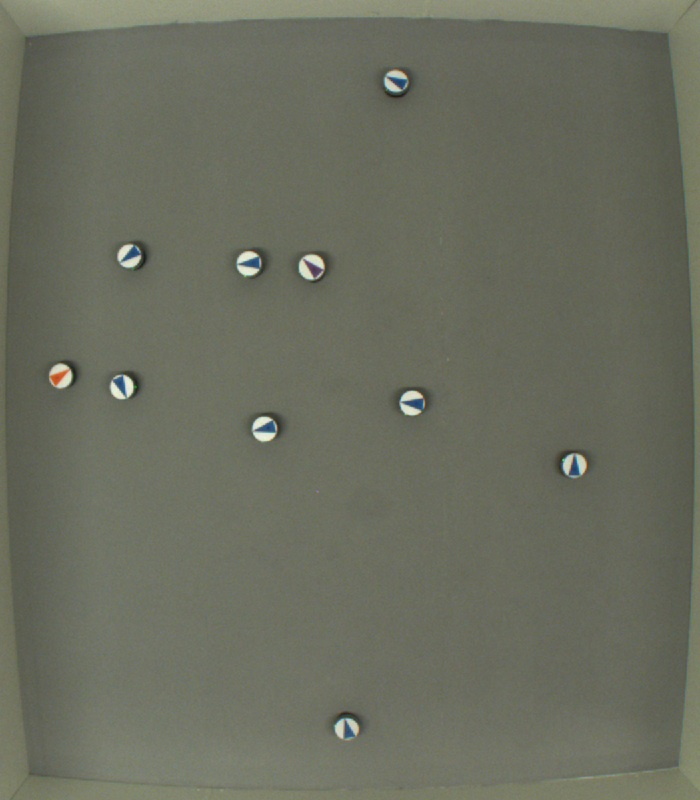
\includegraphics[width=3.0in]{robot_arena.jpg}
    \caption{An image of the robot arena captured by the overhead camera. The robots inside the arena are covered with a colored triangle for facilitating the motion tracking.}
    \label{fig:robot_arena}
\end{figure} 
%
\subsection{Video Processing}

The video processing software was written using OpenCV---an open-source computer vision library~\cite{Gary2008}. The details of the video processing algorithm will be described as follows. 

The image captured using the overhead camera was encoded using RGB. We changed the encoding into HSV in order to make the tracking algorithm less sensitive to lighting variation. This was realized using a built-in function inside the OpenCV library. After that, the image was converted into grayscale and thresholded. As the background of the arena was light-colored, there was no need to do background extraction. After that, we got some binary images. A morphological operation (erosion followed by dilation) is applied on the binary images to filter some noise. Blobs in the binary image with a size above certain threshold (36 pixels) are used for robot detection. These selected blobs indicate the robots in the arena. Fig.~\ref{fig:binary_image_individuals} shows the selected blobs in an image. 
%
\begin{figure}[!t]%
	\centering
		\subfloat[(a) Agents\label{fig:binary_agents}]{%
			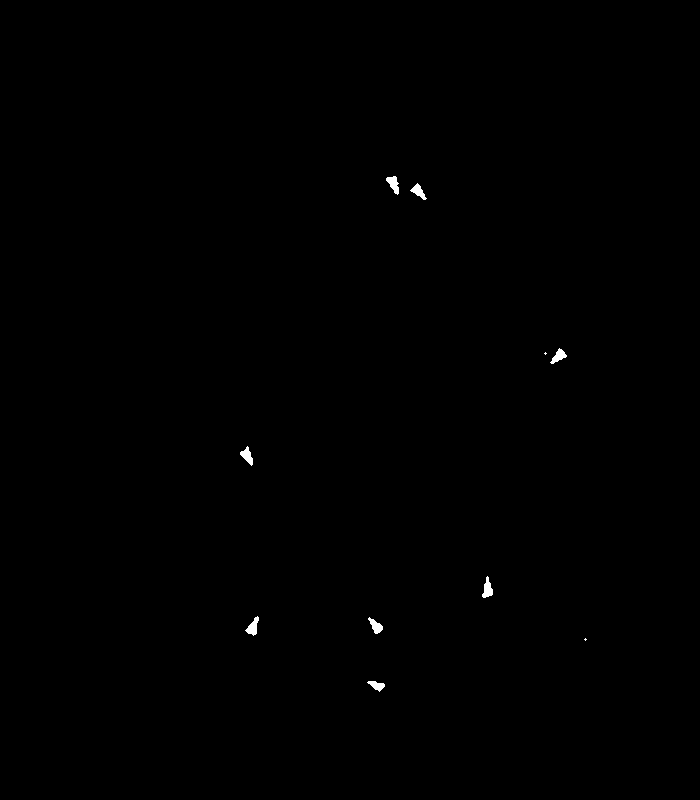
\includegraphics[width=1.65 in]{binary_agents.png} %grid_visualization
		}
		\subfloat[(b) Replica one\label{fig:binary_model_one}]{%
			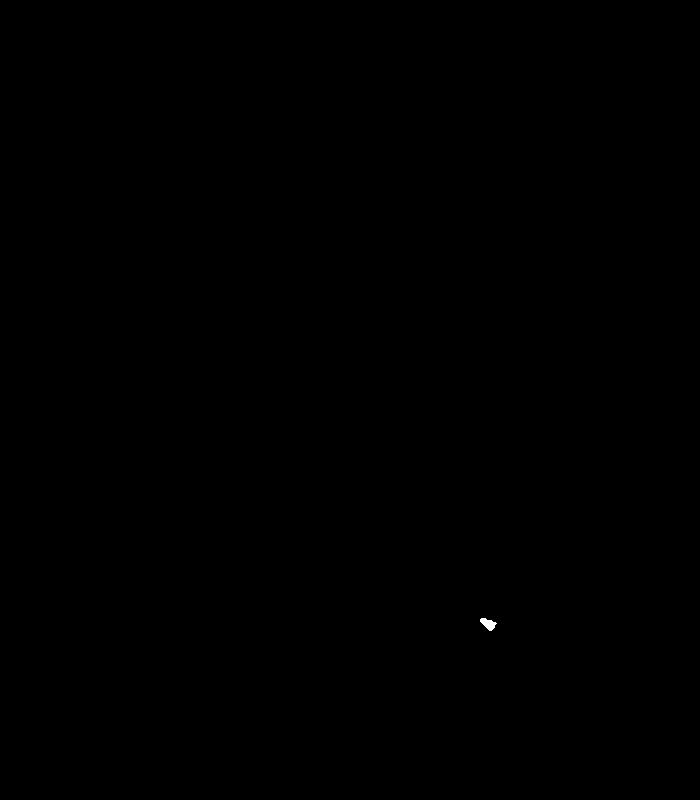
\includegraphics[width=1.65 in]{binary_model_one.png}
		}
		\subfloat[(c) Replica two\label{fig:binary_model_two}]{%
			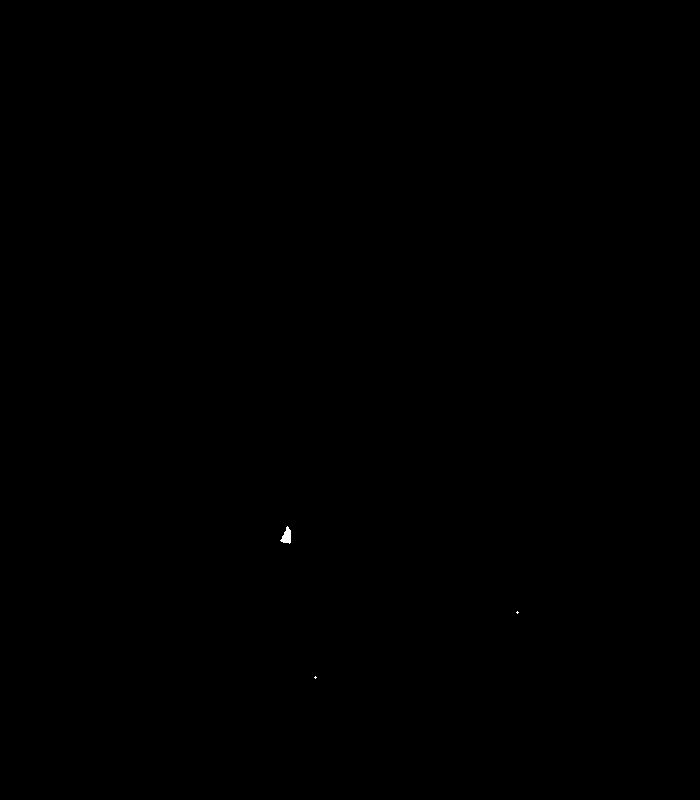
\includegraphics[width=1.65 in]{binary_model_two.png}
		}
		\caption{The images showing the blobs of the robots in the arena. The blobs are selected according to certain compactness and size.}
		\label{fig:binary_image_individuals}
\end{figure}
%

The robots were tracked using the nearest neighbor algorithm. For each blob in the image, we found a minimum triangle that encloses the marker, and got the coordinates of the three vertices of this triangle. The vertex that has the longest distance to the other two vertices indicates the direction of the robot. Therefore the orientation of the robot was estimated using the vector pointing from the midpoint of the other two vertices to this vertex. We use moments~\citep{Hu1962} to calculate the position of the center of the robot. The x and y coordinate of the position is the $1^\mathrm{th}$ order spatial moments around x-axis and y-axis divided by the $0^\mathrm{th}$ order central moments of the blob, respectively. Fig.~\ref{fig:image_processing_flow} shows a diagram of the video processing. 
%
\begin{figure}[!t]
    \centering
    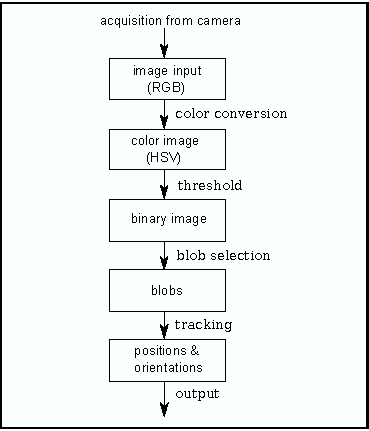
\includegraphics[width=3.5in]{image_processing_flow.pdf}
    \caption{A diagram showing the flow of image processing used in the tracking system.}
    \label{fig:image_processing_flow}
\end{figure} 
%
%
\begin{figure}[!t]
    \centering
    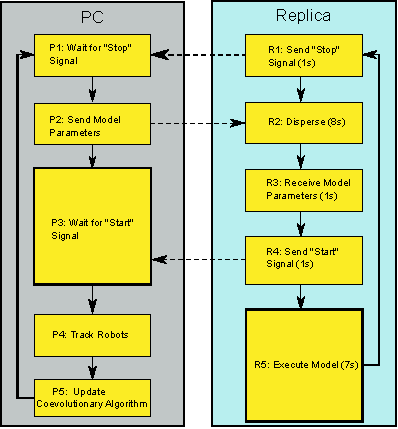
\includegraphics[width=3.5in]{replica_pc_interation.pdf}
    \caption{Schematic of the programs run by the PC and a replica in the physical experiments. Dotted arrows represent communication between the two units. See Sec.~\ref{pc_and_robot_programs} for details.}
    \label{fig:agent_pc_interation}
\end{figure} 
%
\section{PC and Robot Programs}\label{pc_and_robot_programs_swarm_physical}
To automate the coevolutionary process, the PC and robots executed fixed behavioral loops with predefined timings. The PC communicated with the replicas via Bluetooth (we used two replicas to speed up the coevolutionary process, as will be explained in Sec.~\ref{sec:experimental_protocol}) . This served for the PC to issue the replicas with models to be executed, and to synchronize the PC with the swarm. The agents did not perform any communication. At the start of a coevolution run, or after a human intervention (see Sec.~\ref{sec:experimental_protocol}), robots were synchronized using an infrared signal from a remote control.

Fig.~\ref{fig:agent_pc_interation} shows a schematic of the programs run by the PC and the replicas. These programs are represented in terms of various states, with dotted arrows indicating communication between the units. The agents executed a similar behavioral loop to the replicas. Next, we detail the states of the programs executed by the PC, replicas, and agents.

\subsection{PC Program}
\begin{itemize}
	\item \textit{P1:} \textit{Wait for ``Stop'' Signal.} The program is halted until ``Stop'' signals are received from the replicas. These signals indicate that a trial has finished.
	
	\item \textit{P2:} \textit{Send Model Parameters.} The PC sends new model parameters to each replica. These go to the replicas' buffers as the replicas are still in state \textit{R2}; they are later read by the replicas in state \textit{R3}.
	
	\item \textit{P3:} \textit{Wait for ``Start'' Signal.} The program is halted until ``Start'' signals are received from the replicas, indicating that a trial is starting.
	
	\item \textit{P4:} \textit{Track Robots.} The PC waits one second and starts tracking the robots' motion using the overhead camera. While the trial is run for seven seconds (see \textit{R5}), tracking is only performed during the middle five, to discard potentially noisy data from the beginning and end.
	
	\item \textit{P5:} \textit{Update Coevolutionary Algorithm.} The PC performs a fitness update step in the coevolutionary algorithm. The motion data from the trial observed in \textit{P4} is used to update the fitness of the corresponding two models and all the classifiers (according to the procedure described in Chapter~\ref{ch:swarm_simulation}. If all models in the current generation have been evaluated, the PC also generates new model and classifier populations. The PC then goes back to \textit{P1}.
\end{itemize}

\subsection{Replica Program}
\begin{itemize}

\item \textit{R1}: \textit{Send ``Stop'' Signal.} After a trial stops, the replica informs the PC by sending a ``Stop'' signal. 
The PC sends a new model to the replica's buffer.
The replica waits one second before moving to \textit{R2}, so that all robots remain synchronized (agents are programmed to restart one second after a trial stops). Waiting one second in other states serves the same purpose.

\item\textit{R2}: \textit{Disperse.} The replica disperses in the environment, while avoiding collisions with other robots and the walls. This behavior lasts eight seconds.

\item\textit{R3}: \textit{Receive Model Parameters.} The replica reads new model parameters from its buffer (sent earlier by the PC). It waits one second before moving to \textit{R4}.

\item\textit{R4}: \textit{Send ``Start'' Signal.} The replica sends a start signal to the PC to inform it that a trial is about to start. The PC prepares to start tracking the robots' motion. The replica waits one second before moving to \textit{R5}.

\item\textit{R5}: \textit{Execute Model.} The replica moves within the swarm according to its model. This behavior lasts seven seconds. The replica then moves back to \textit{R1}.
\end{itemize}
%A video showing a cycle of the sequential behaviors for the agents and replicas as well as the implementation details of \textit{R2} can be found in the online supplementary material~\cite{online_supplementary_material_tevc2014}.

\subsection{Agent Program}
\begin{itemize}
\item The agents follow the same behavioral loops as the replicas. However, in the states analogous to \textit{R1}, \textit{R3}, and \textit{R4}, they simply wait one second rather than communicate with the PC. In the state corresponding to \textit{R2}, they also execute the \textit{Disperse} behavior. In the state corresponding to \textit{R5}, they execute the real aggregation controller, rather than a model.
\end{itemize}

\section{Experimental Setup and Protocol}\label{sec:experimental_protocol_swarm_physical}
In the coevolutionary algorithm, we used population sizes of $20$ for models, and $100$ for classifiers (as opposed to $100$ models in the simulated coevolutions of Chapter~\ref{ch:swarm_simulation}; this was done to reduce experimental time). We used $10$ robots in the arena: $8$ representing agents executing the real aggregation controller (Eq.~\eqref{eq:aggregation_optimal_controller}), and $2$ representing replicas that executed models. This meant that in each trial, $2$ models from the population could be evaluated simultaneously; consequently, each generation consisted of $20/2=10$ trials. 
%Note from the previous section that each trial lasted $\unit[18]{s}$; each generation therefore lasted $10\times 18 = \unit[180]{s}$. We chose to run coevolutions for $100$ generations, for a total time of around $5$ hours per run (excepting human interventions).

The coevolutionary algorithm was implemented without any modification to the code used in simulation (except for model population size and observation time in each trial). We still let the model parameters evolve unboundedly (i.e., in $\mathbb{R}^4$). However, as the speed of the physical robots is naturally bounded, we applied the hyperbolic tangent function ($\tanh{x}$) on each model parameter, before sending a model to a replica. This bounded the parameters to $\left(-1,1\right)^4$, with $-1$ and $1$ representing the maximum backward and forward wheel speeds, respectively.

During a coevolution run, a human intervention was made in the following cases. Otherwise, the run proceeded autonomously.
\begin{itemize}
\item The robots had been running continuously for $25$ generations. All batteries were replaced.

\item A robot stopped moving, for example because of a lost battery connection or because it became stuck on the floor. Appropriate action was taken for the affected robot.

\item A replica lost its Bluetooth connection with the PC. The connection (with both replicas) was restarted.

\item A robot indicated a low battery status through its LED after running for only a short time. That robot's battery was changed.
\end{itemize}

After an intervention, the ongoing generation was restarted, to limit the impact on the coevolutionary process.

%In each situation, either the batteries or robots were changed. To limit the impact on the evaluation, the current generation was rerun. %, otherwise the robots would stop working for the rest of trials 

%In order to reduce the chances of robots getting stuck on the wall (note that the aggregation behavior was designed in an unbounded environment), the aggregation behavior was modified. When the robot detected the wall using the four proximity sensors in its back (sensors 2, 3, 4, 5 in Fig.~\ref{fig:e_puck_schematic}), it behaved as if $I=1$ (for example,  the agent would turn on the spot). This action was only triggered when the sensory value was above a certain threshold. Since the robots were covered with a black `skirt', the value of the proximity sensors was very low when two robots were near each other, therefore this action did not affect the aggregation behavior. 
%
\begin{figure}[!t]
    \centering
    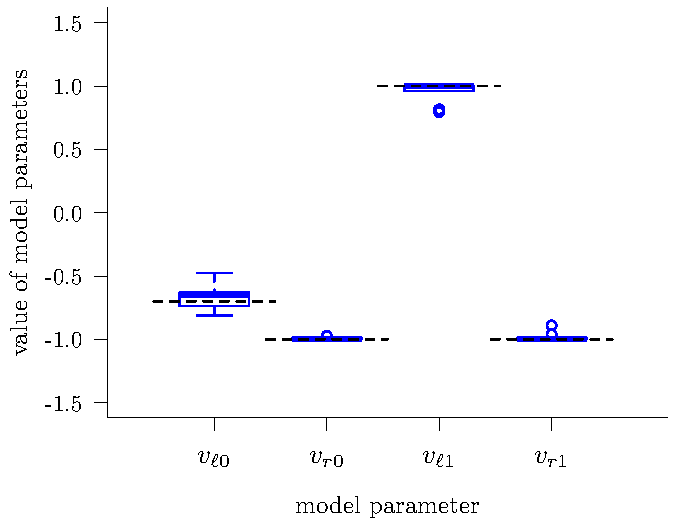
\includegraphics[width=3.5in]{best_model_parameters_physical.pdf}
    \caption{Parameters of the evolved models in the $100^{\textrm{th}}$ generation of $10$ physical coevolution runs. Dotted black lines indicate true values.}
    \label{fig:best_model_parameters_physical}
\end{figure}
%
\section{Results}\label{sec:experimental_results_swarm_physical}
We conducted $10$ coevolution runs using the physical system. Each run lasted $100$ generations, corresponding to around $5$ hours (excluding human intervention time).
%
%Note from the previous section that each trial lasted $\unit[18]{s}$; each generation therefore lasted $10\times 18 = \unit[180]{s}$. We chose to run coevolutions for $100$ generations, for a total time of around $5$ hours per run (excepting human interventions).
\begin{figure}[!t]%
	\centering
		\subfloat[(a) Simulated Coevolutions\label{fig:model_parameters_convergence_compare_simulation}]{%
			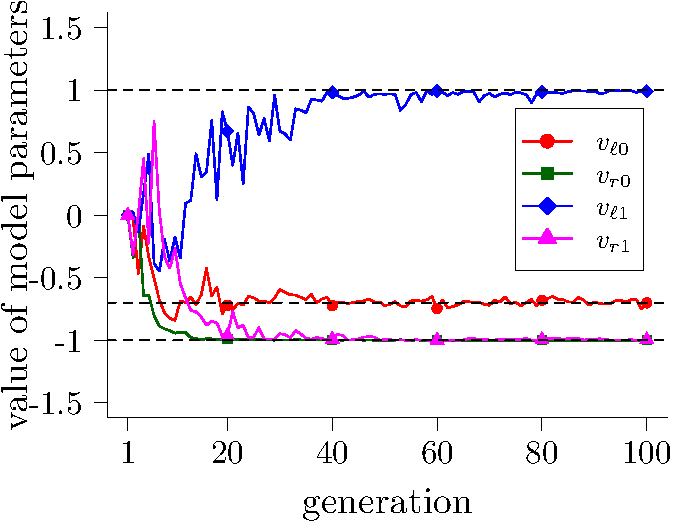
\includegraphics[width=3.5 in]{model_parameters_convergence_compare_simulation.pdf} %grid_visualization
		}\\
		\subfloat[(b) Physical Coevolutions\label{fig:model_parameters_convergence_compare_physical}]{%
			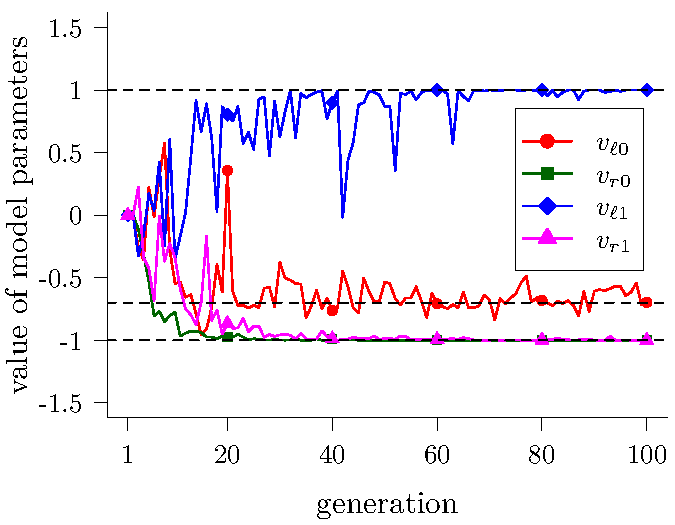
\includegraphics[width=3.5 in]{model_parameters_convergence_compare_physical.pdf}
		}
		\caption{Evolutionary progress of each model parameter in $10$ (a) simulated and (b) physical coevolution runs. Curves represent median values across $10$ runs. Dotted black lines indicate true values.}
		\label{fig:model_parameters_convergence_compare}
\end{figure}
%
\subsection{Post Evaluation}
 To select the `best' model from each coevolution run, we post-evaluated all evolved models in the final generation $5$ times using all classifiers in that generation. The parameters of these models are shown in Fig.~\ref{fig:best_model_parameters_physical}. The means (standard deviations) of the AEs in each parameter were: $0.08$ ($0.06$), $0.01$ ($0.01$), $0.05$ ($0.08$), and $0.02$ ($0.04$).

To investigate the effects of real-world conditions on the coevolutionary method, we performed $10$ simulated coevolution runs with the same setup as in the physical runs.
Fig.~\ref{fig:model_parameters_convergence_compare} shows the evolutionary dynamics of the evolved model parameters in the simulated and physical coevolution runs.
Figures~\subref*{fig:model_parameters_convergence_compare_simulation}  and~\subref*{fig:model_parameters_convergence_compare_physical} show that the dynamics show good correspondence overall. However, the convergence in the physical coevolutions is somewhat less smooth than that in the simulated ones (e.g., the spikes in $v_{\ell0}$ and $v_{l1}$). One reason for this may be the limitations in motion data capture and extraction. In particular, given the relatively small diameter of the e-puck in our arena, inferring its orientation is particularly challenging.

We will now investigate the classifiers' performance. In each generation 
of every coevolution run (simulated and physical), we computed the MAE of each model. We compared the error of the model with the highest subjective fitness with the average and lowest errors. The results are shown in Fig.~\ref{fig:MAE_compare_simulation_physical}.
In both the simulated and physical cases, the subjectively best model (green) has an error in between the average (red) and the lowest (blue) in the majority of generations. Also in both cases the gap between the error of the subjectively best model and the average error becomes wider as the coevolution proceeds, which means the classifiers are only misguided by increasingly good models. This gap, in turn, forces the model population to evolve, as indicated by the downwards trend of the lowest error.
%
% Fig.~\subref*{fig:model_parameters_convergence_compare_physical}, the error of the models with the highest objective fitness is becoming smaller until about $60^\textrm{th}$ generation, and then it increases slightly. We suspect that this is due to the fact that when the replica behaves more like the agents (that is, the model parameters converge to their real value), it is more likely to collide with them (i.e., to aggregate). the chance of its collision with other agents is higher than those replicas that executes `worse' models.
%
\begin{figure}[!t]%
	\centering
		\subfloat[(a) Simulated Coevolutions\label{fig:MAE_simulation}]{%
			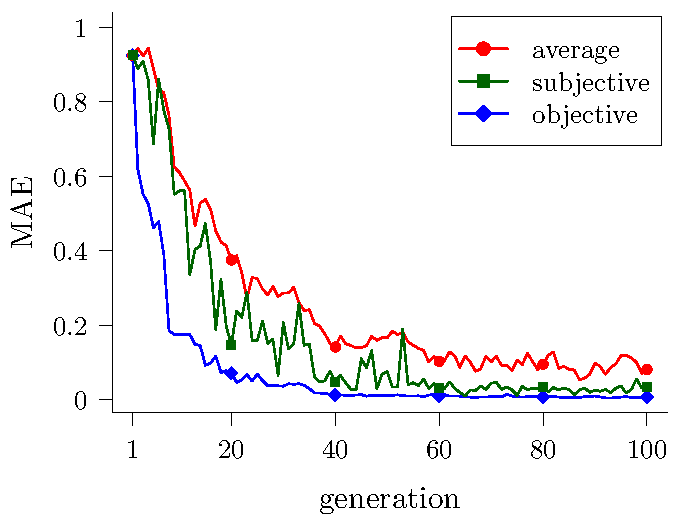
\includegraphics[width=3.5 in]{MAE_simulation.pdf} %grid_visualization
		}\\
		\subfloat[(b) Physical Coevolutions\label{fig:MAE_physical}]{%
			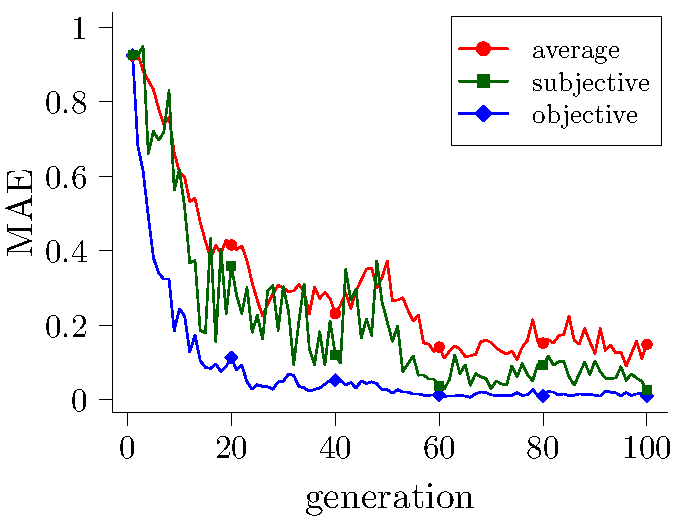
\includegraphics[width=3.5 in]{MAE_physical.pdf}
		}
		\caption{Evolutionary progress of models in $10$ (a) simulated and (b) physical coevolution runs. Curves represent median values across $10$ runs. The red curve represents the average error of all models in a generation. The green and blue curves show, respectively, the errors of the models with the highest subjective and the highest objective fitness in a generation.}
		\label{fig:MAE_compare_simulation_physical}
\end{figure}
%
\begin{figure}[!t]
    \centering
    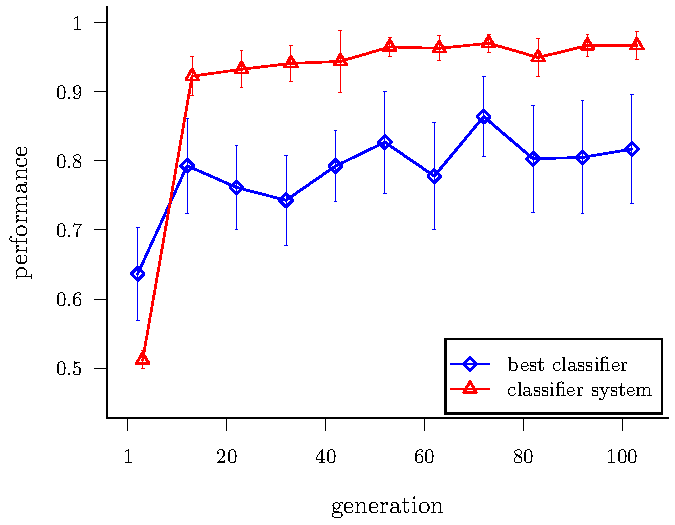
\includegraphics[width=3.5in]{all_generation_judgment_accuracy_physical.pdf}
    \caption{Average performance of the classifier system selected using the recording data during the trials over $10$ coevolution runs. The error bar shows standard deviation.}
    \label{fig:all_generation_judgment_accuracy_physical}
\end{figure}

In order to further investigate the performance of the classifier system (as discussed in details in Chapter~\ref{ch:swarm_simulation}), we evaluated the evolved classifiers in every $10$ generation using $100$ models\footnote{Note that since it takes too long to perform a grid evaluation as we did in simulation, here we only evaluated the performance of the classifiers using a limited number of random-generated models.}. The parameters of each model were randomly-generated in $[-1,1]^4$. For the details of the selection process of the classifier system, refer to Chapter~\ref{ch:swarm_simulation}. Fig.~\ref{fig:all_generation_judgment_accuracy_physical} shows the performance of the best classifier and the classifier system over generations. Similar to the results obtained in simulation, the classifier system evolved in the physical coevolution runs still has a high performance over the testing individuals (including agents and models). However, in contrast to simulation, the performance of the best classifier did not drop with the increasing generations. This may be due to the reason that it took longer for the models to converge in the physical coevolutionary experiments and the best classifier selected according to the available recording data was not over-specialized as in the simulation. 

\subsection{Model Validation}
As we argued before (Sec.~\ref{sec:analysis_evolved_models}), in swarm systems, good agreement between local behaviors (e.g., controller parameters) is not a guarantee of similar global behaviors. For this reason, we performed $20$ trials using $40$ e-pucks, lasting $10$ minutes each: $10$ with the real controller (Eq.~\eqref{eq:aggregation_optimal_controller}), and $10$ with a controller obtained from the physical coevolution runs. This latter controller was constructed by taking the median values of the parameters over the $10$ runs, which are:
$$
\mathbf{p}=\left(-0.65, -0.99, 0.99, -0.99\right).
$$
The set of initial configurations of the robots was common to both controllers. As it was not necessary to extract the orientation of the robots, a red circular marker was attached to each robot so that its position can be extracted with good accuracy in the offline analysis.
%
\begin{figure}[!t]%
	\centering
		\subfloat[(a) Largest Cluster Dynamics \label{fig:aggregation_dynamics_proportion}]{
			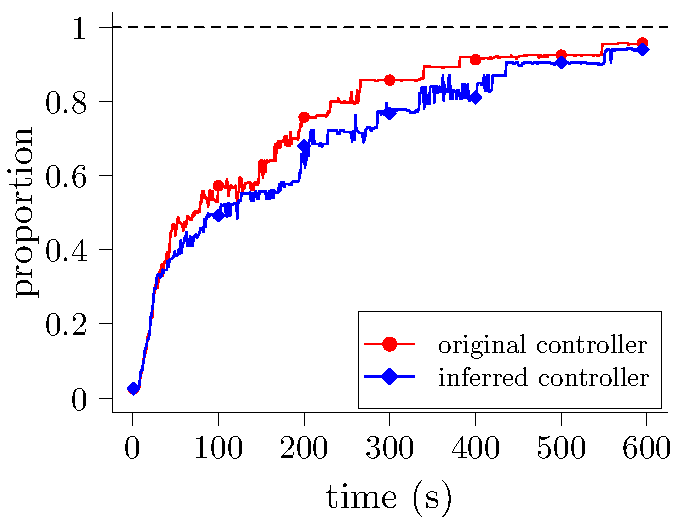
\includegraphics[width=3.5 in]{aggregation_dynamics_proportion.pdf}
		}\\
		\subfloat[(b) Dispersion Dynamics \label{fig:aggregation_dynamics_compactness}]{
			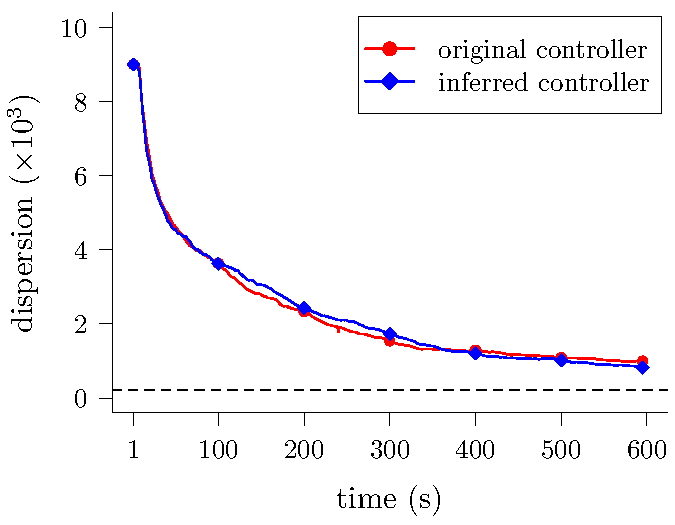
\includegraphics[width=3.5 in]{aggregation_dynamics_compactness.pdf}
		}
		\caption{Average aggregation dynamics in $10$ physical trials with $40$ e-puck robots executing the real controller (red) and the evolved controller (blue). In (a), the vertical axis shows the proportion of robots in the largest cluster; in (b), it shows the robots' dispersion (see Sec.~\ref{sec:analysis_evolved_models}). Dotted lines in (a) and (b), respectively, represent the maximum proportion and minimum dispersion that $40$ robots can achieve.}
		\label{fig:aggregation_dynamics_physical}
\end{figure}
%
Fig.~\subref*{fig:aggregation_dynamics_proportion} shows the proportion of robots in the largest cluster\footnote{A cluster of robots is defined as a maximal connected subgraph of the graph defined by the robots' positions, where two robots are considered to be adjacent if another robot cannot fit between them~\cite{Gauci2014_ijrr}.} over time with the real and evolved controllers. Fig.~\subref*{fig:aggregation_dynamics_compactness} shows the dispersion (as defined in Sec.~\ref{sec:analysis_evolved_models}) of the robots over time with the two controllers. The aggregation dynamics of the real and evolved behaviors show good correspondence. Fig.~\ref{fig:aggregation_snapshoot_physical_validation} shows a sequence of snapshots from a trial with $40$ e-pucks executing the evolved controller.

\begin{figure}[!t]
\centering
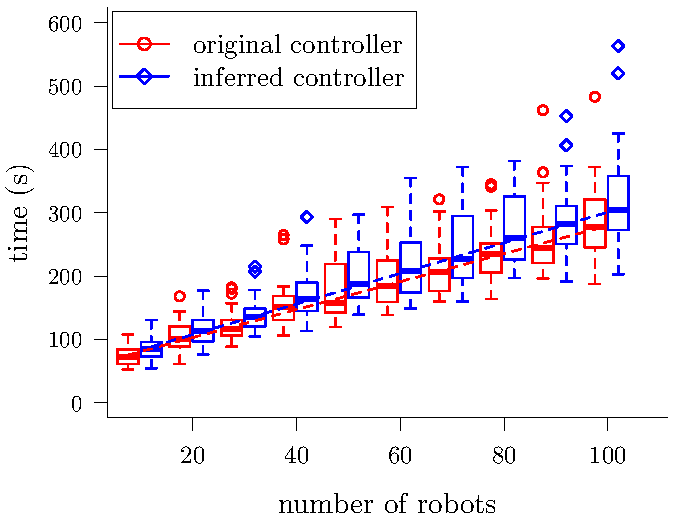
\includegraphics[width=3.5in]{aggregation_model_validation_physical.pdf}
\caption{Time taken for different numbers of robots to aggregate into a single cluster. Each box corresponds to $30$ simulation trials with the real controller (red), and the controller obtained from the physical coevolution runs (blue).}
\label{fig:aggregation_model_validation_physical}

\end{figure}

\captionsetup[subfigure]{labelformat=empty}  
\begin{figure*}[!t]
	\centering
	\subfloat[initial configuration]{
		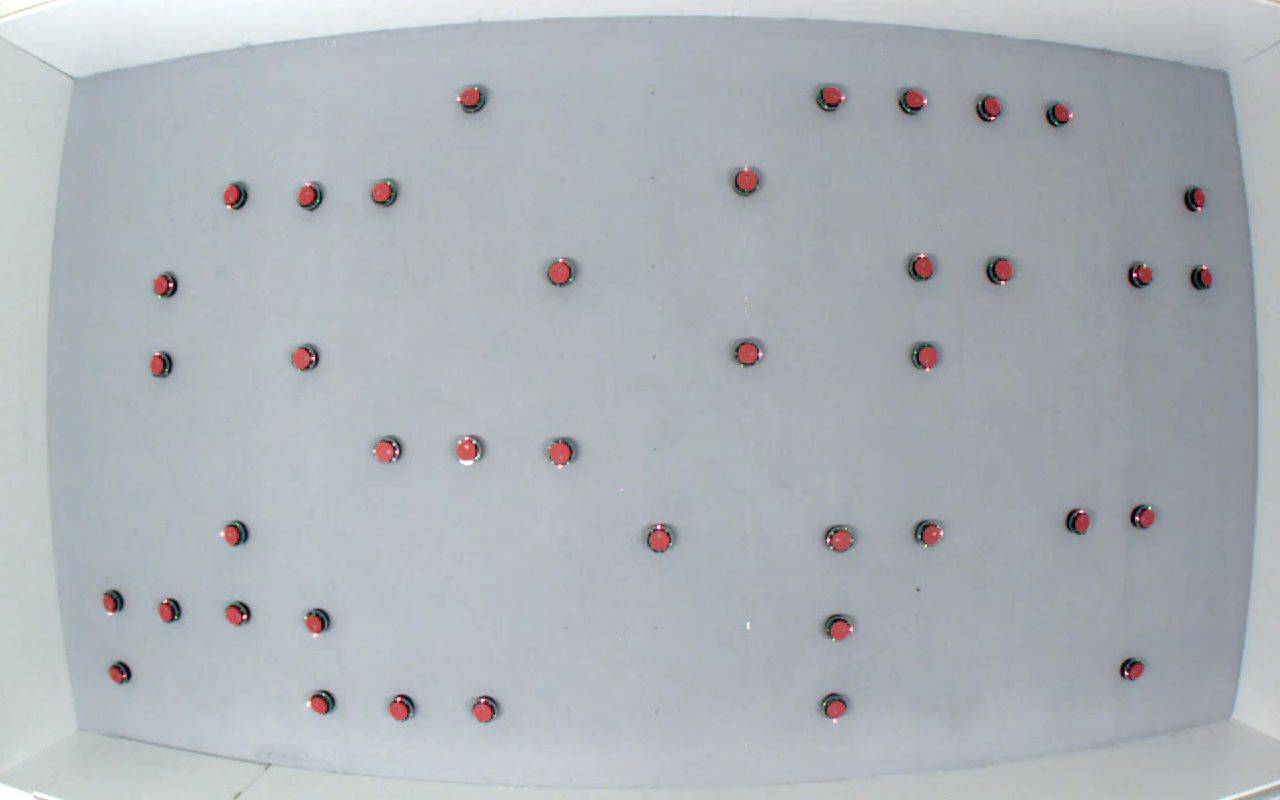
\includegraphics[width = 1.7 in]{physical_snapshot_0s.jpg}
	}
	\subfloat[after $20$ $\unit{s}$]{
		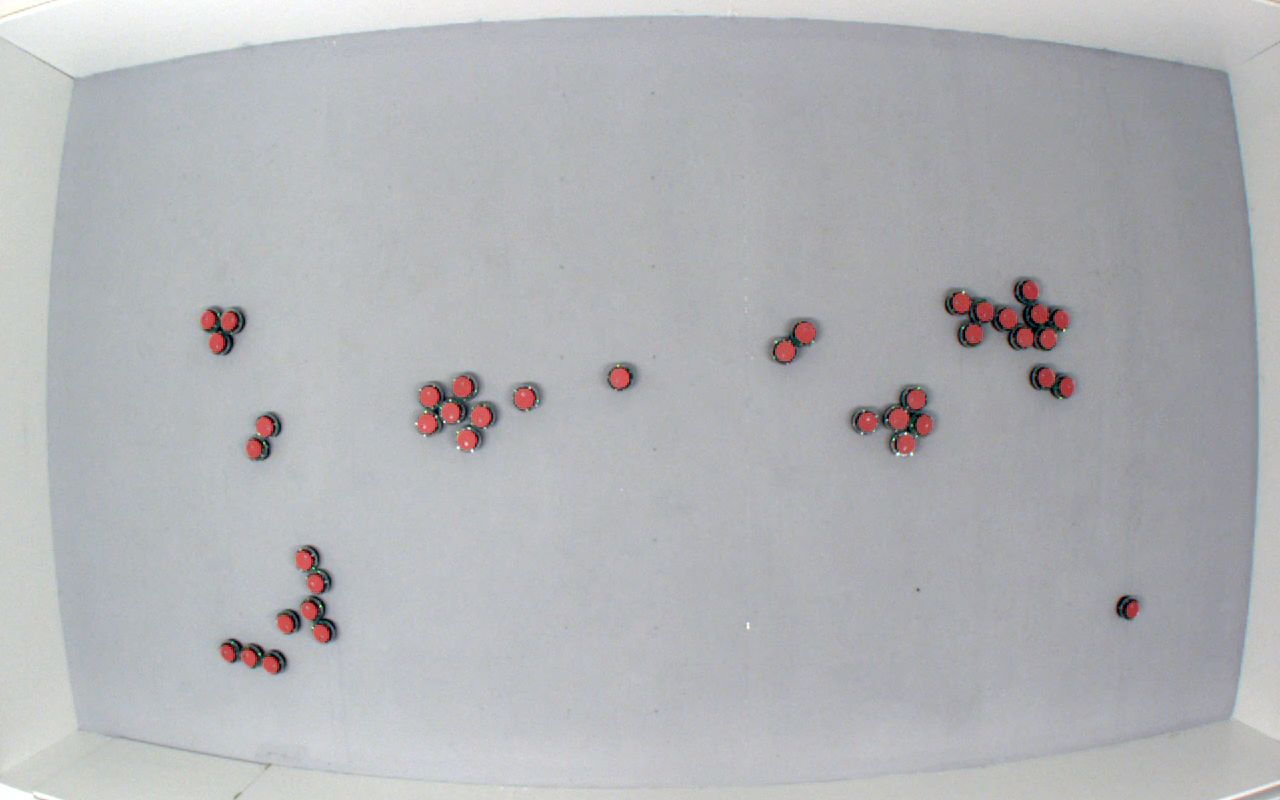
\includegraphics[width = 1.7 in]{physical_snapshot_20s.jpg}
	}\\
	\subfloat[after $40$ $\unit{s}$]{
		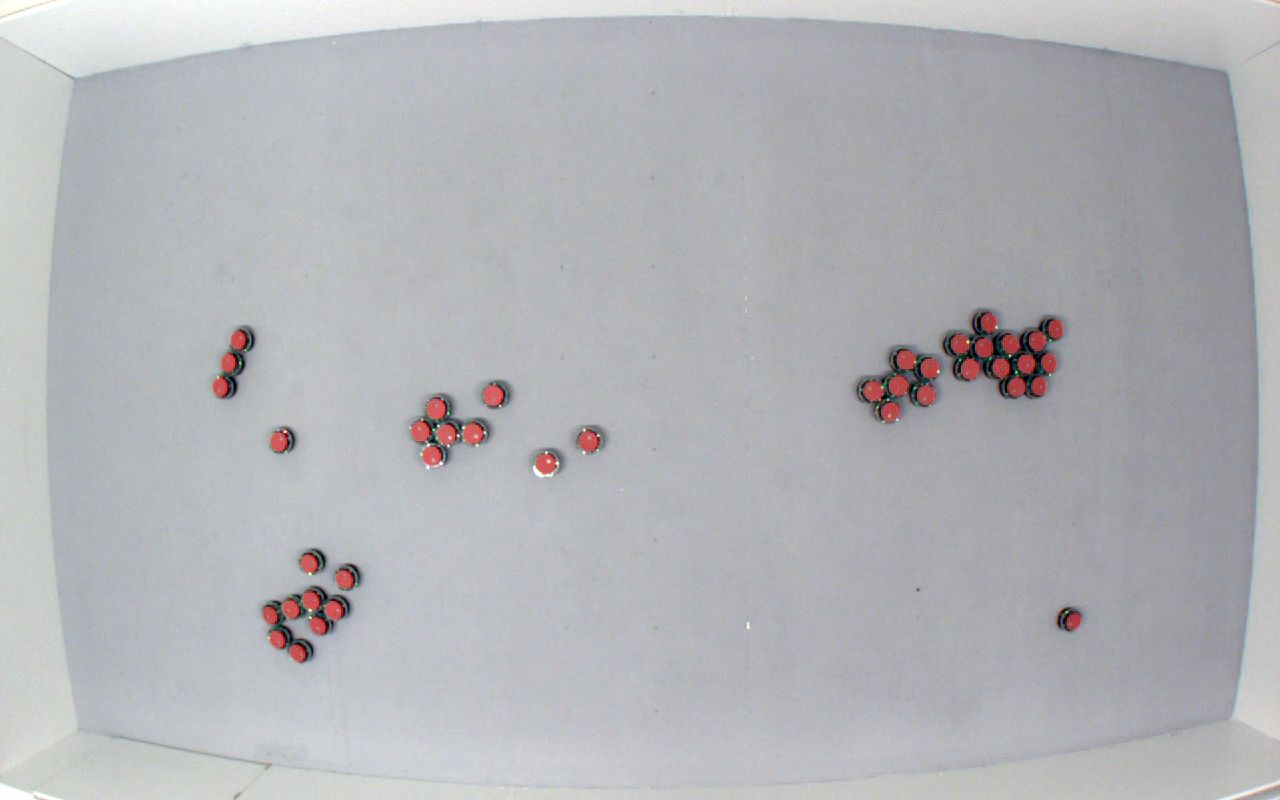
\includegraphics[width = 1.7 in]{physical_snapshot_40s.jpg}
	}
	\subfloat[after $180$ $\unit{s}$]{
		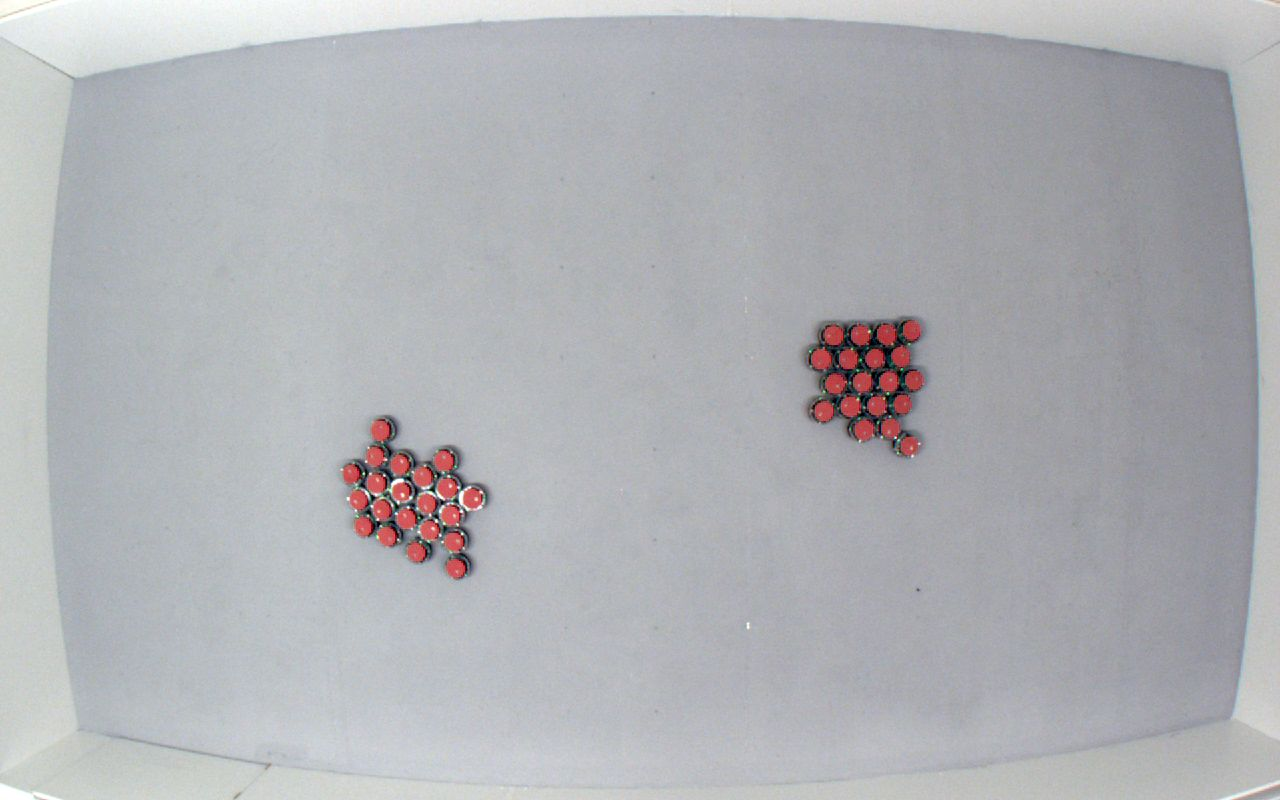
\includegraphics[width = 1.7 in]{physical_snapshot_180s.jpg}
	}\\
		\subfloat[after $360$ $\unit{s}$]{
		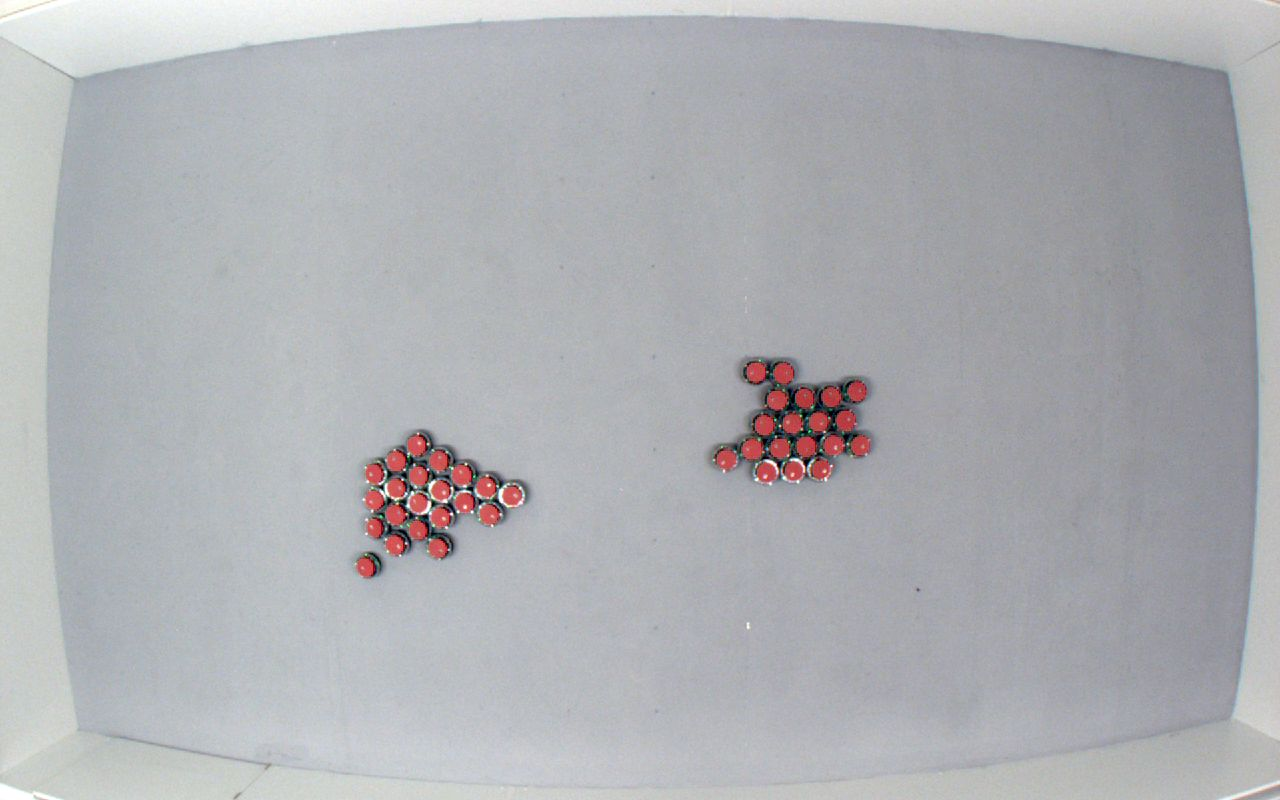
\includegraphics[width = 1.7 in]{physical_snapshot_360s.jpg}
	}
	\subfloat[after $420$ $\unit{s}$]{
		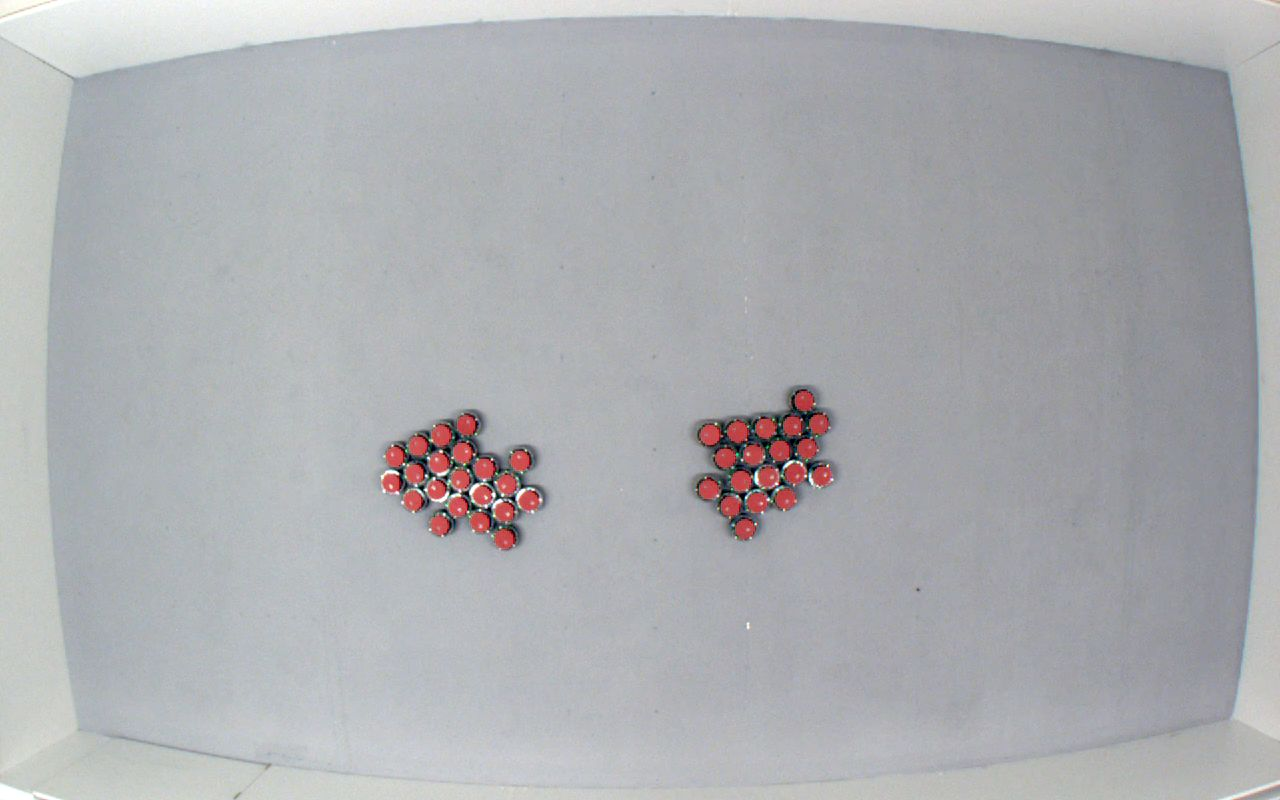
\includegraphics[width = 1.7 in]{physical_snapshot_420s.jpg}
	}\\
	\subfloat[after $480$ $\unit{s}$]{
		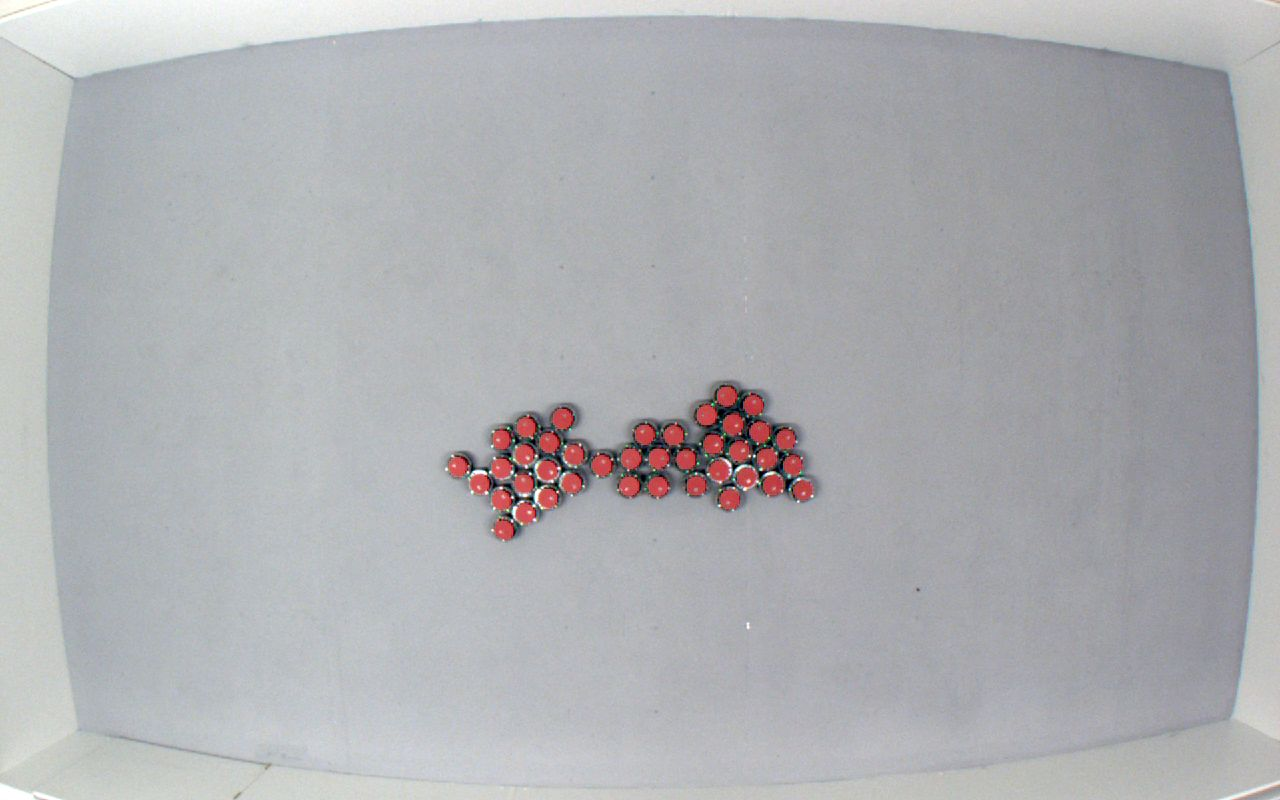
\includegraphics[width = 1.7 in]{physical_snapshot_480s.jpg}
	}
	\subfloat[after $600$ $\unit{s}$]{
		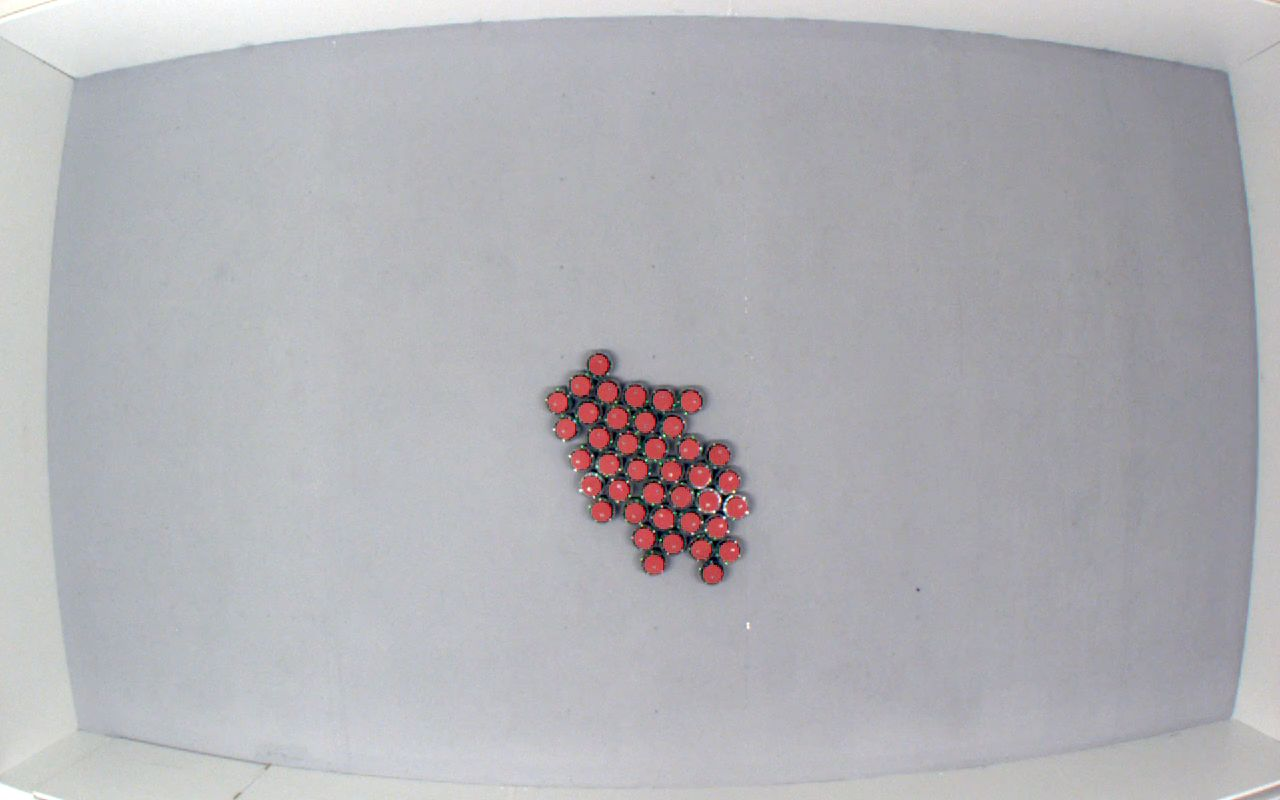
\includegraphics[width = 1.7 in]{physical_snapshot_600s.jpg}
	}
	\caption{Snapshots of the aggregation behavior with $40$ e-puck robots using the model that was automatically learned through observation of swarms of physical robots in the coevolution.}
	\label{fig:aggregation_snapshoot_physical_validation}
\end{figure*}

We also performed a scalability study in simulation to compare the real and evolved controllers. We calculated the time taken to form a single cluster with different numbers of robots: $n \in \lbrace10, 20, \dots, 100\rbrace$. For each number of robots, we performed $30$ trials with each controller. The results are shown in Fig.~\ref{fig:aggregation_model_validation_physical}. In all cases, the real controller slightly outperforms the evolved one.
However, with either controller, the robots aggregate in a relatively short time ($<\unit[600]{s}$). There is a statically significant difference in aggregation times with the two controllers for $n= 10, 30, 50, 70, 80, 90$---but this suggests no particular pattern with respect to $n$. We also performed a linear least squares regression on the aggregation times with the two controllers. The fits were: $T = 53.2 + 2.2n$ for the real controller, and $T = 64 + 2.4n$ for the evolved controller ($n>1$). This indicates that the evolved controller does not scale much worse than the real one.

The video accompanying this paper shows the evolutionary process both in simulation and on the physical system. It also shows the emergent, global behaviors of the real controller and the obtained model on the physical system. Additionally, videos of all $10$ physical coevolution runs, and all $20$ post-evaluation trials with $40$ e-pucks, are available in the online supplementary material~\cite{online_supplementary_material_tevc2014}.

\begin{figure}[!t]
    \centering
    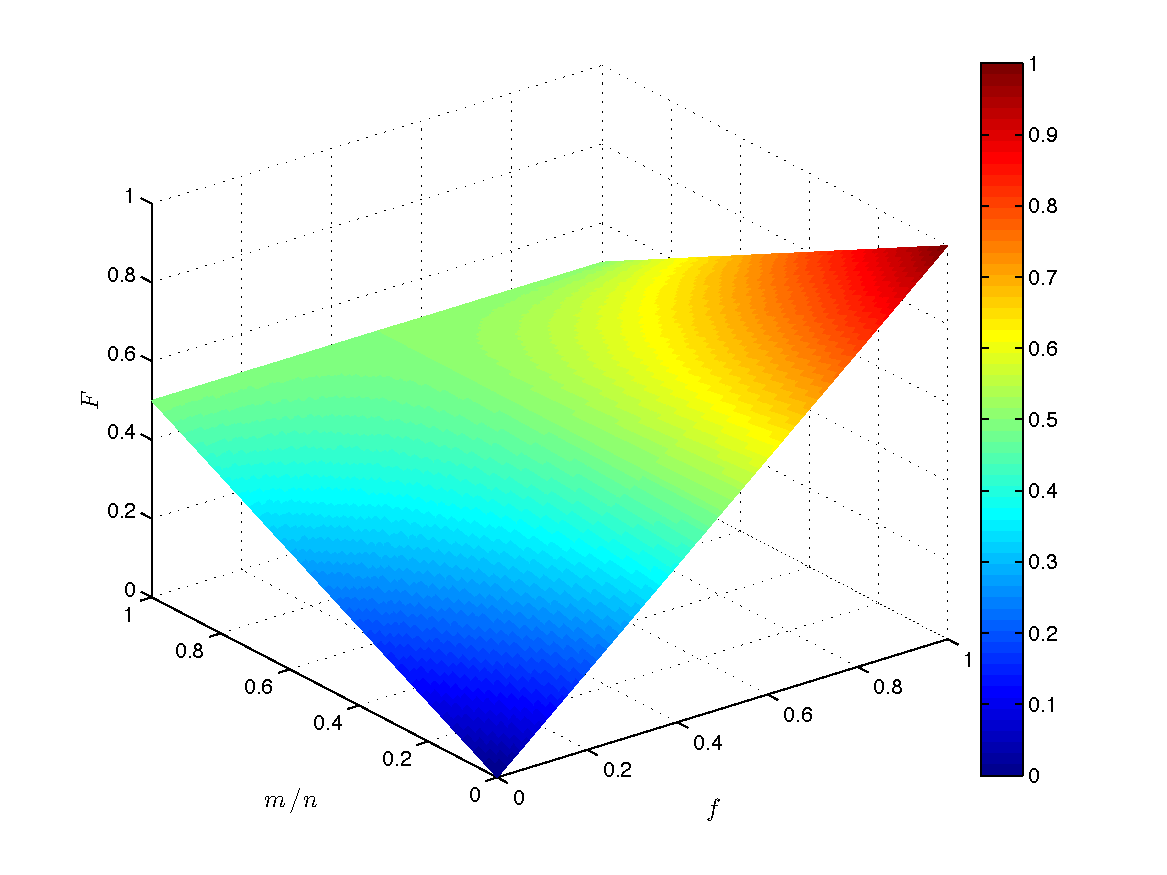
\includegraphics[width=3.5in]{algorithm_sensitivity_analysis.pdf}
    \caption{This plot shows the relationship between the old fitness, $f$, and the new fitness, $F$, of the classifiers, when the failure ratio of agents in the swarm, $\frac{m}{N}$, changes. When $m = 0$ or $N \rightarrow \infty$, $F=f$. When $0 < \frac{m}{N} < 1$, $F$ is shifted, but the fitness order is not changed.}
    \label{fig:analysis_algorithm}
\end{figure}

\section{Analysis of Sensitivity for Individual Failure}\label{sec:analysis_algorithm}

In the physical experiments, we have observed that some robots may get stuck or stop working because of the reasons mentioned in Section~\ref{sec:experimental_protocol}. This could also happen in a real swarm system, for example, some individuals may stop moving or display other abnormal behaviors due to various factors such as collision. These abnormal behaviors (which are considered failure here) may not be recognized during the process of experiments. Therefore, we have analyzed whether abnormal behaviors (failure) of some individuals may bias the evolution and hence affect performance of our proposed coevolutionary approach. Assuming the failure is equally likely to be present in the replica and agent in a trial. We have proved that: \textit{\textbf{the metric-free coevolutionary approach is not biased by failure of certain individuals in the swarm.}} The mathematical proof is provided as follows:
 
\begin{proof}
Let $n$ be the total size of the group, consisting of $n-1$ agents and $1$ replica. $m$ represents the number of individuals that fail ($m<n$) in a trial. $p$ and $q$ are the probabilities of a classifier to make the correct judgment for models and agents respectively. Therefore, the expected fitness of the classifier without failure of any individuals in one generation, $f_c$, is equal to $\frac{p+q}{2}$. $f_m$ denotes the fitness of a model in that generation. 

There are two failure cases: 1) failure with the replica; 2) failure without the replica. We assume that if an individual fails during a trial, the classifier makes random judgment, that is, it has equal probability, which is $50\%$, of judging the individual as an agent or a model. If failure exists in a trial, the probability that failure with the replica occurs, $p_1$, is as follows:
\begin{equation}
{p_1} = {\binom{n-1}{m-1}} / {\binom{n}{m}} = \frac{m}{n}.
\end{equation}
The probability that failure without the replica occurs in a trial, $p_2$, is: $1 - p_1 = \frac{n-m}{n}$. The proof is divided into two parts: one for the classifiers and the other is for models.

For the classifier, the new fitness in the first failure case, $f_{c1}$, can be calculated as follows:
\begin{equation}\label{equ:f1:classifier}
{f_{c1}} = p_1 \cdot (\frac{1}{2} + \frac{1}{2} \cdot \frac{m-1}{n-1} + \frac{q \cdot (n-m)}{n-1}) /2.
\end{equation}
In the second failure case, the new fitness of the classifier, $f_{c2}$, is given by:
\begin{equation}\label{equ:f2:classifier}
{f_{c2}} = p_2 \cdot (p + \frac{1}{2} \cdot \frac{m}{n-1} + \frac{q \cdot (n-m-1)}{n-1}) / 2.
\end{equation}
Combining Eqs.~\eqref{equ:f1:classifier} and~\eqref{equ:f2:classifier} and simplifying the resulting expression, the new fitness, $F_c$, of the classifier when $m$ individuals fail in a trial is:
\begin{equation}\label{equ:F:classifier}
{F_c} = f_{c1} + f_{c2} = f_c \cdot (1-\frac{m}{n}) + \frac{m}{2n}.
\end{equation}

In Eq.\eqref{equ:F:classifier}, $F_c$ is monotonic increasing in terms of $f_c$. When $f_c$, is equal to $0.5$, $F_c$ maintains the same value. When $f_c$ is greater than (or smaller than) $0.5$, $F_c$ is decreased (or increased) but still greater (or smaller) than $0.5$. Therefore, the fitness order of all the classifiers after failure of $m$ individuals in a trial is not changed, which means it does not affect the selection of the classifiers in the evolutionary process. 
%http://www.numberempire.com/simplifyexpression.php Fig.~\ref{fig:analysis_algorithm} visualized how the fitness of the classifiers is shifted when failure of agents occurs. %{F_c} = f_{c1} + f_{c2} = \frac{m}{2N}[1 + (p + q) \cdot \frac{N-m}{m}] = f \cdot (1-\frac{m}{N}) + \frac{m}{2N}.

For the model, it has a new fitness of $f_{m1} = \frac{m}{n} \cdot \frac{1}{2}$ and $f_{m2} = \frac{(n-m) \cdot f_m}{n}$ in the first and second failure case, respectively. Therefore, the new fitness of the model, $F_m$, when $m$ individuals fail in a trial is:
\begin{equation}\label{equ:F:model}
{F_m} = f_{m1} + f_{m2} = f_m \cdot (1-\frac{m}{n}) + \frac{m}{2n}.
\end{equation}
Comparing Eqs.~\eqref{equ:F:classifier} and~\eqref{equ:F:model}, we can see that the fitness order of all the models is also unchanged when failure occurs in a trial.
\end{proof}

\section{Summary}\label{sec:summary_swarm_physical}

In this chapter, we presented a physical autonomous coevolutionary system for identifying the aggregation behavior in Chapter~\ref{ch:swarm_simulation} using swarms of e-puck robots. The behavior was learned successfully, and the results obtained in the physical experiments show good correspondence to those obtained in simulation. This showed the robustness of our metric-free coevolutionary method with respect to noise and uncertainties in real world, which provided a first step towards automated reversing engineering of  swarm behaviors with little human intervention~\cite{King2009, Schmidt2009}. 

The model obtained in the physical coevolution runs was validated using $40$ e-puck robots. The global behavior of the obtained model is similar to that of the real controller. The selected classifier system over the coevolution runs still obtained a high performance, which means our classifier system could be potentially applied to detect or monitor the behaviors of the agents in a swarm. 
% The step of validation is necessary in our approach. As the classifiers only observed the motion of each individual, and were not provide any information about the global behaviors of the agents. One case that could happen is the evolved model parameters are similar to those of the agents, but the global behaviors of the models and agents are different. 

In order to speed up the coevolutionary process, different from simulation, we used two replicas instead of one. Therefore, two models can be executed simultaneously. In principle, we could further speed up the process through using more replicas in parallel. However, considering the reliability of communication between the replicas and PC as well as the influence of replicas on the whole swarm behaviors, a limited number of replicas is recommended. 

We have proved that our coevolutionary approach is robust to failure of individuals in the mixed group. That is, even if some individuals failed during the trials, this won't bias the results we get. This highlights our metric-free approach as the metric-based approach may be biased due to some individual exceptional behaviors.

